\documentclass[a4paper, 14pt]{extarticle}%тип документа

%Русский язык
\usepackage[T2A]{fontenc} %кодировка
\usepackage[utf8]{inputenc} %кодировка исходного кода
\usepackage[english,russian]{babel} %локализация и переносы

%отступы 
\usepackage[left=2cm,right=2cm,top=2cm,bottom=3cm,bindingoffset=0cm]{geometry}

%Вставка картинок
\usepackage{graphicx}
\usepackage{wrapfig, caption}
\graphicspath{}
\DeclareGraphicsExtensions{.pdf,.png,.jpg, .jpeg}
\newcommand\ECaption[1]{%
     \captionsetup{font=footnotesize}%
     \caption{#1}}

%Таблицы
\usepackage[table,xcdraw]{xcolor}
\usepackage{booktabs}

%Графики
\usepackage{pgfplots}
\pgfplotsset{compat=1.9}

%Математика
\usepackage{amsmath, amsfonts, amssymb, amsthm, mathtools}

%Заголовок
\author{Подлесный Артём \\ группа 827}
\title{Работа 3.4.2 \\ Закон Кюри-Вейсса}

\begin{document}
\maketitle
\paragraph*{Цель работы: }
изучение температурной зависимости магнитной восприимчивости ферромагнетика выше точки Кюри.
\paragraph*{Оборудование: }
катушка самоиндукции с образцом из гадолиния, термостат, частотомер, цифровой вольтметр, LC-автогенератор, термопара медь-константин.
\section*{ Отчёт о работе}
\subsection*{Общая теория}
Вещества с отличными от нуля атомными магнитными моментами обладают парамагнитными свойствами. Внешнее магнитное поле ориентирует магнитные моменты, которые в отсутствие поля располагались в пространстве хаотичным образом.

При повышении температуры $T$ магнитная восприимчивость парамагнетиков убывает. В постоянном магнитном поле по закону Кюри:
\begin{equation}
\chi = \frac{C}{T},
\end{equation}
где $C$ -- постоянная Кюри.
\newpage
\begin{wrapfigure}{l}{0.3\textwidth}
\begin{center}
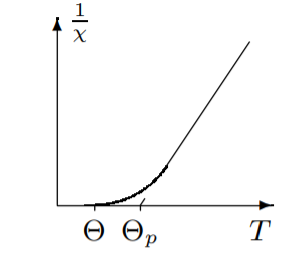
\includegraphics[height=3cm]{teor.png}
\end{center}
\ECaption{Зависимость обратной величины магнитной восприимчивости от температуры}
\end{wrapfigure}

Для парамагнитных веществ, которые при понижении температуры становятся ферромагнитными, формула (1) может быть видоизмененна. При $T \longrightarrow 0$  тепловое движение всё меньше препятствует магнитным моментам атомов ориентироваться в одном направлении при сколь угодно малом поле. В ферромагнетиках -- под влиянием обменных сил -- это происходит при понижении температуры не до абсолютного нуля, а до температуры Кюри $\Theta$. Оказывается, что у ферромагнетиков закон Кюри должен быть заменён законом Кюри-Вейсса:
\begin{equation}
\chi\sim\dfrac{1}{T - \Theta_{p}},
\end{equation}
где $\Theta_{p}$ -- температура, близкая к температуре Кюри.
\subsection*{Экспериментальная установка}
\begin{figure}[h!]
\begin{center}
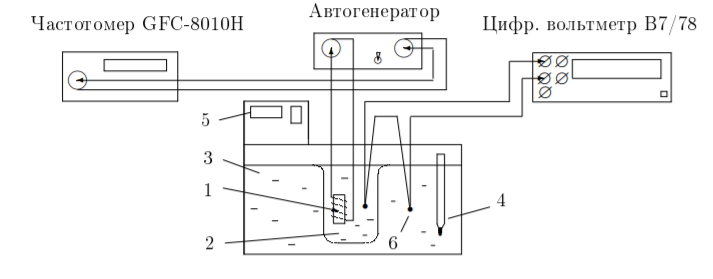
\includegraphics[width=0.8\textwidth]{ust}
\end{center}
\ECaption{Экспериментальная установка}
\end{figure}
При изменении температуры образца меняется и его магнитная восприимчивость $\chi$, а следовательно самоиндукция катушки и период колебаний $\tau$ автогенератора. Для измерения периода используется частотометр.

Температура исследуемого образца всегда несколько отличается от температуры воды в сосуде. Разность их температур контролируется с помощью термопары и электронного вольтметра. Период колебаний автогенератора измерялся, когда эта разность становилась $\leq 0.5^{\circ} C$. Чувствительность термопары: $k = 24 \text{ град/мВ}$. Соответственно допустимое значение напряжения на вольтметре: $\Delta U = 21\text{ мкВ}$.
\subsection*{Экспериментальные данные}
Была исследованна зависимость колебаний LC-генератора от температуры образца. Измерялись: $\tau$ -- период колебаний, $T_d$ -- показания температуры на дисплее термостата, $\Delta U$ -- ЭДС термопары (с учетом знака). Отсюда была посчитана температура образца $T$ по формуле:
\[T = T_d + k\Delta U,\]
Зависимость показана на таблице. Период колебаний без образца $\tau_0 = 6.9092$.
% Please add the following required packages to your document preamble:
% \usepackage[table,xcdraw]{xcolor}
% If you use beamer only pass "xcolor=table" option, i.e. \documentclass[xcolor=table]{beamer}
\begin{table}[h!]
\begin{tabular}{|l|l|l|l|l|l|}
\hline
\rowcolor[HTML]{FFC702} 
$\tau \text{, мкc}$            & $T_d\text{, C}$             & $\Delta U \text{, мкВ}$       & $T$, $C^{\circ}$                       & $\tau^2 -\tau_0^2$, $\text{мкc}^2$    & $\dfrac{10^3}{\tau^2 - \tau_0^2}$, $\text{мкc}^{-2}$ \\ \hline
7.92795                        & 15.22                       & 3                           & 15.15                        & 15.12                        & 66.16                                      \\ \hline
\rowcolor[HTML]{FFFFC7} 
7.85581                         & 17.08                       & 22                          & 16.55                        & 31.97                        & 31.28                                      \\ \hline
7.70161                         & 19.11                       & 18.3                        & 18.67                        & 50.83                        & 19.67                                      \\ \hline
\rowcolor[HTML]{FFFFC7} 
{\color[HTML]{333333} 7.44928} & {\color[HTML]{333333} 21.1} & {\color[HTML]{333333} 18.6} & {\color[HTML]{333333} 20.65} & {\color[HTML]{333333} 71.68} & {\color[HTML]{333333} 13.95}               \\ \hline
7.27881                        & 23.1                        & 14.4                        & 22.75                        & 94.54                        & 10.58                                      \\ \hline
\rowcolor[HTML]{FFFFC7} 
7.17764                        & 25.08                       & 20.1                        & 24.60                        & 119.39                       & 8.38                                       \\ \hline
7.12139                        & 27.09                       & 19.1                        & 26.63                        & 146.25                       & 6.84                                       \\ \hline
\rowcolor[HTML]{FFFFC7} 
7.08831                        & 29.08                       & 18.8                        & 28.63                        & 175.11                       & 5.71                                       \\ \hline
7.06676                        & 31.07                       & 19.9                        & 30.59                        & 205.96                       & 4.86                                       \\ \hline
\rowcolor[HTML]{FFFFC7} 
7.0502                        & 33.07                       & 17.3                        & 32.65                        & 238.82                       & 4.19                                       \\ \hline
7.0385                        & 35.07                       & 16.4                        & 34.68                        & 273.67                       & 3.65                                       \\ \hline
\rowcolor[HTML]{FFFFC7} 
7.0225                        & 37.07                       & 16.9                        & 36.66                        & 310.53                       & 3.22                                       \\ \hline
7.0216                        & 39.06                       & 18.1                        & 38.63                        & 349.39                       & 2.86                                       \\ \hline
\rowcolor[HTML]{FFFFC7} 
7.0161                        & 41.07                       & 6.1                         & 40.92                        & 390.24                       & 2.56                                       \\ \hline
\end{tabular}
\end{table}

Погрешность в определении $\Delta U$ составляла 0.3 мкВ, в определении $T_d$ - 0.03 К, $\tau$ - 0.00012 мкс. Исходя из этого были посчитанны погрешности для всех остальных значений.
\subsection*{Обработка экспериментальных данных}
Необходимо определить парамагнитную точку Кюри $\Theta_p$. Для этого построим графики следующей зависимости: $(\tau^2 - \tau_0^2)^{-1} = f(T)$.
\begin{figure}[h!]
\center{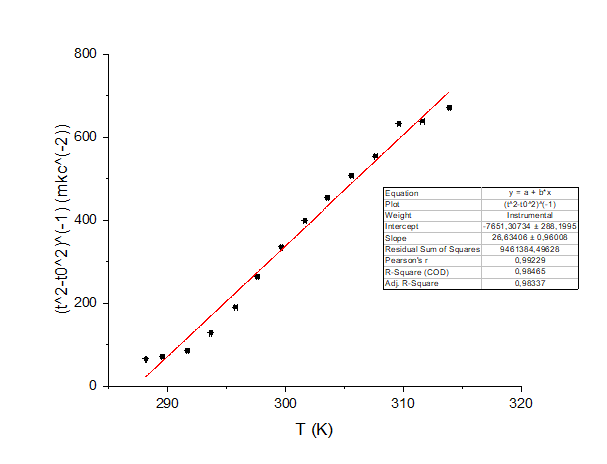
\includegraphics[scale=1.2]{gr2.png}}
\caption{Зависимость $(\tau^2 - \tau_0^2)^{-1} = f(T)$.}
\end{figure}
Экстраполируя график, находим пересечение графика с осью абсцисс. Отсюда, используя погрешности коэффициента угла наклона графика и знач пересечения с осью ординат, получаем результат для парамагнитной температуры Кюри:
\begin{equation}
\Theta_p = \dfrac{Intercept}{Slope} = (287 \times 15) \text{ K.}
\end{equation}
Табличное значение температуры Кюри для гадолиния составляет
\begin{equation}
\Theta_{pteor} = 290 \text{ K.}
\end{equation}
Отсюда видно, что найденное значение соотвествует табличному с учетом погрешности.

\section*{ Вывод}
Таким образом была изучена температурная зависимость магнитной восприимчивости ферромагнетика выше точки Кюри. Было показано, что эта зависимость носит характер парамагнетика, и для нее выполняется закон Кюри-Вейсса, тк с большой точностью определена парамагнитная точка Кюри, которая совпадает с табличным значением.












\end{document}